\documentclass[11pt,compress,t,notes=noshow]{beamer}\usepackage[]{graphicx}\usepackage[]{color}

\makeatletter
\def\maxwidth{ %
  \ifdim\Gin@nat@width>\linewidth
    \linewidth
  \else
    \Gin@nat@width
  \fi
}
\makeatother

\definecolor{fgcolor}{rgb}{0.345, 0.345, 0.345}
\newcommand{\hlnum}[1]{\textcolor[rgb]{0.686,0.059,0.569}{#1}}%
\newcommand{\hlstr}[1]{\textcolor[rgb]{0.192,0.494,0.8}{#1}}%
\newcommand{\hlcom}[1]{\textcolor[rgb]{0.678,0.584,0.686}{\textit{#1}}}%
\newcommand{\hlopt}[1]{\textcolor[rgb]{0,0,0}{#1}}%
\newcommand{\hlstd}[1]{\textcolor[rgb]{0.345,0.345,0.345}{#1}}%
\newcommand{\hlkwa}[1]{\textcolor[rgb]{0.161,0.373,0.58}{\textbf{#1}}}%
\newcommand{\hlkwb}[1]{\textcolor[rgb]{0.69,0.353,0.396}{#1}}%
\newcommand{\hlkwc}[1]{\textcolor[rgb]{0.333,0.667,0.333}{#1}}%
\newcommand{\hlkwd}[1]{\textcolor[rgb]{0.737,0.353,0.396}{\textbf{#1}}}%
\let\hlipl\hlkwb

\usepackage{framed}
\makeatletter
\newenvironment{kframe}{%
 \def\at@end@of@kframe{}%
 \ifinner\ifhmode%
  \def\at@end@of@kframe{\end{minipage}}%
  \begin{minipage}{\columnwidth}%
 \fi\fi%
 \def\FrameCommand##1{\hskip\@totalleftmargin \hskip-\fboxsep
 \colorbox{shadecolor}{##1}\hskip-\fboxsep
     \hskip-\linewidth \hskip-\@totalleftmargin \hskip\columnwidth}%
 \MakeFramed {\advance\hsize-\width
   \@totalleftmargin\z@ \linewidth\hsize
   \@setminipage}}%
 {\par\unskip\endMakeFramed%
 \at@end@of@kframe}
\makeatother

\definecolor{shadecolor}{rgb}{.97, .97, .97}
\definecolor{messagecolor}{rgb}{0, 0, 0}
\definecolor{warningcolor}{rgb}{1, 0, 1}
\definecolor{errorcolor}{rgb}{1, 0, 0}
\definecolor{code}{rgb}{0.97, 0.96, 1.0}
\newenvironment{knitrout}{}{} % an empty environment to be redefined in TeX

\usepackage{alltt}
\usepackage[utf8]{inputenc}
\usepackage[ngerman]{babel}
\usepackage{dsfont}
\usepackage{verbatim}
\usepackage{amsmath}
\usepackage{amsfonts}
\usepackage{mathtools}
\usepackage{csquotes}
\usepackage{cmbright}
\usepackage{multirow}
\usepackage{longtable}
\usepackage{enumerate}
\usepackage[absolute,overlay]{textpos}
\usepackage{psfrag}
\usepackage{algorithm}
\usepackage{algpseudocode}
\usepackage{eqnarray}
\usepackage{bytefield}
\usepackage{animate}
\usepackage{tikz}
\usetikzlibrary{shapes,matrix,positioning,chains,arrows,shadows,decorations.pathmorphing,fit,backgrounds}
\usepackage{adjustbox}
\usepackage{colortbl}
\usepackage{tabularx} % for tables (incl. \hline)
\usepackage{arydshln} % Load after array, longtable, colortab and/or colortbl , otherwise problems with \hline in tabular env
\usepackage{etex} %increase registers for \dimenS to more than 256, otherwise we get "No room for a new \dimen"
\usepackage{graphicx}
\usepackage{booktabs} %used in epr lectures
\usepackage{bm} % bold greek letters
\usepackage{hyperref} % url citing
\usepackage{blkarray} % block arrays
\usepackage{listings} % block of code
\usepackage{xcolor} %colored math symbols
\usepackage{pgffor}
\usepackage{verbatimbox}
\usepackage{xcolor}

%some colors
\definecolor{checkgreen}{HTML}{18A126}
\definecolor{errorred}{HTML}{FF0000}
\definecolor{blockbg}{HTML}{F7F7F7}
\definecolor{gray}{HTML}{A0A0A0}

% basic latex stuff
\newcommand{\col}{\par\colorbox{code}{\parbox{\textwidth}{\theverbbox}}\par}
\newcommand{\eg}{e.\,g.\xspace} %for example
\newcommand{\ie}{i.\,e.\xspace} %that is to say...
\newcommand{\pkg}[1]{{\fontseries{b}\selectfont #1}} %fontstyle for R packages
\newcommand{\lz}{\vspace{0.5cm}} %vertical space
\newcommand{\oneliner}[1] % Oneliner for important statements
{\begin{block}{}\begin{center}\begin{Large}#1\end{Large}\end{center}\end{block}}
\def\SpAr{\quad \Rightarrow \quad}

%new environments
\newenvironment{vbframe}  %frame with breaks and verbatim
{
 \begin{frame}[containsverbatim,allowframebreaks]
}
{
\end{frame}
}

\newenvironment{vframe}  %frame with verbatim without breaks (to avoid numbering one slided frames)
{
 \begin{frame}[containsverbatim]
}
{
\end{frame}
}

\newenvironment{blocki}[1]   % itemize block
{
 \begin{block}{#1}\begin{itemize}
}
{
\end{itemize}\end{block}
}

\newenvironment{fragileframe}[2]{  %fragile frame with framebreaks
\begin{frame}[allowframebreaks, fragile, environment = fragileframe]
\frametitle{#1}
#2}
{\end{frame}}

\newcommand{\myframe}[2]{  %short for frame with framebreaks
\begin{frame}[allowframebreaks]
\frametitle{#1}
#2
\end{frame}}

\usepackage{../../style/lmu-lecture}

\let\code=\texttt
\let\proglang=\textsf

\setkeys{Gin}{width=0.9\textwidth}

\usepackage{tikz}
\usetikzlibrary{shapes,arrows,snakes, calc}

% Define block styles
\tikzstyle{decision} = [diamond, draw, text width=6em, text badly centered, node distance=4cm, inner sep=0pt]
\tikzstyle{decision2} = [diamond, draw, fill=customgreen!35, text width=6em, text badly centered, node distance=4cm, inner sep=0pt]

\tikzstyle{block} = [rectangle, draw, text width=14em, text centered, rounded corners, node distance=3cm, minimum height=4em]
\tikzstyle{line} = [draw, -latex']
\tikzstyle{cloud} = [draw, ellipse, node distance=3cm, minimum height=2em]

\title{Introduction to Deep Learning}
\author{Bernd Bischl}
\institute{Department of Statistics -- LMU Munich}
\date{WS 2021/2022}

\setbeamertemplate{frametitle}{\expandafter\uppercase\expandafter\insertframetitle}

\IfFileExists{upquote.sty}{\usepackage{upquote}}{}
\input{../../latex-math/basic-math}
\input{../../latex-math/basic-ml}
\input{../../latex-math/ml-nn}

\newcommand{\titlefigure}{figure/spiral_planar_data/he_intro.png}
\newcommand{\learninggoals}{
  \item 
  \item 
  \item 
}

\title{Deep Learning}
\date{}

\begin{document}

\lecturechapter{Network Initializations}
\lecture{I2DL}

%%%%%%%%%%%%%%%%%%%%%%%%%%%%%%%%%%%%%%%%%%%%%%%%%%%%%%%%%%%%%%%%%%
\begin{vbframe} {Practical Initialization}
  \begin{itemize}
    \item The weights (and biases) of a neural network must be assigned some initial values before training can begin.
    \item The choice of the initial weights (and biases) is crucial as it determines whether an optimization algorithm converges, how fast and whether to a point with high or low risk. 
    \item Initialization strategies to achieve "nice" properties are difficult to find, because there is no good understanding which properties are preserved under which circumstances. 
    \item In the following we seperate between the initialization of weights and biases. 
  \end{itemize}
  \end{vbframe}
  
%%%%%%%%%%%%%%%%%%%%%%%%%%%%%%%%%%%%%%%%%%%%%%5
\begin{vbframe}{Weight Initialization}
  \begin{itemize}
    \item It is important to initialize the weights randomly in order to "break symmetry". If two neurons (with the same activation function in a fully connected network) are connected to the same inputs and have the same initial weights, then both neurons will have the same gradient update in a given iteration and they will end up learning the same features.
    \item Furthermore, the initial weights should not be too large, because this might result in an explosion of weights or high sensitivity to changes in the input.
    \item Weights are typically drawn from a uniform distribution or a Gaussian centered at 0 with a small variance.
    \item Centering the initial weights around 0 can be seen as a form of regularization and it imposses that it is more likely that units do not interact with each other than they do interact.
    \framebreak
    \item Two common initialization strategies for weights are the 'Glorot initialization' and 'He initialization' which tune the variance of these distributions based on the topology of the network. %However, these strategies depend on the layer size and the initial weights can get extremely small with larger layer sizes.
    \item \textbf{Glorot initialization} suggests to sample each weight of a fully connected layer with $m$ inputs and $n$ outputs from a uniform distribution
    \begin{equation*}
      w_{j,k} \sim U\left(-\sqrt{\frac{6}{m+n}},\sqrt{\frac{6}{m+n}}\right)
    \end{equation*}
   The strategy is derived from the assumption that the network consists only of a chain of matrix multiplications with no nonlinearities. 
    \item \textbf{He initialization} is especially useful for neural networks with ReLU activations. Each weight of a fully connected layer with $m$ inputs is sampled from a Gaussian distribution 
    \begin{equation*}
      w_{j, k} \sim N\left(0, \frac{2}{m}\right)
    \end{equation*}
    The underlying derivation can be found in He et. al. (2015).
    \item Since the initialization strategies of Glorot and He depend on the layer sizes, the initial weights for large layer sizes can become extremely small.
    \item Another strategy is to treat the weights as hyperparameters that can be optimized by hyperparameter search algorithms. This can be computationally costly. 
    %\item Another strategy is to manually search for optimal weights by looking at the range or standard deviations of activations and gradients on a single minibatch. If the weights are too small, the range of the activations shrinks and the weights should be manually increased.
  \end{itemize}
\end{vbframe}

%%%%%%%%%%%%%%%%%%%%%%%%%%%%%%%%%%%%%%%%%%%%%%%%%%%%%%%%%%%%%%%%%%
\begin{vbframe}{Weight initialization: Example}
\begin{itemize}
\item We use a spiral planar data set to compare the following strategies: \\
Zero initialization, random initialization (samples from $N\left(0, 1\cdot 10^{-4}\right)$) and He initialization. 
\item For each strategy, a neural network with one hidden layer with 100 units, ReLU activation and Gradient Descent as optimizer was used. 
\end{itemize}
  \begin{figure}
  \vspace{-0.5cm}
    \centering
      \scalebox{0.4}{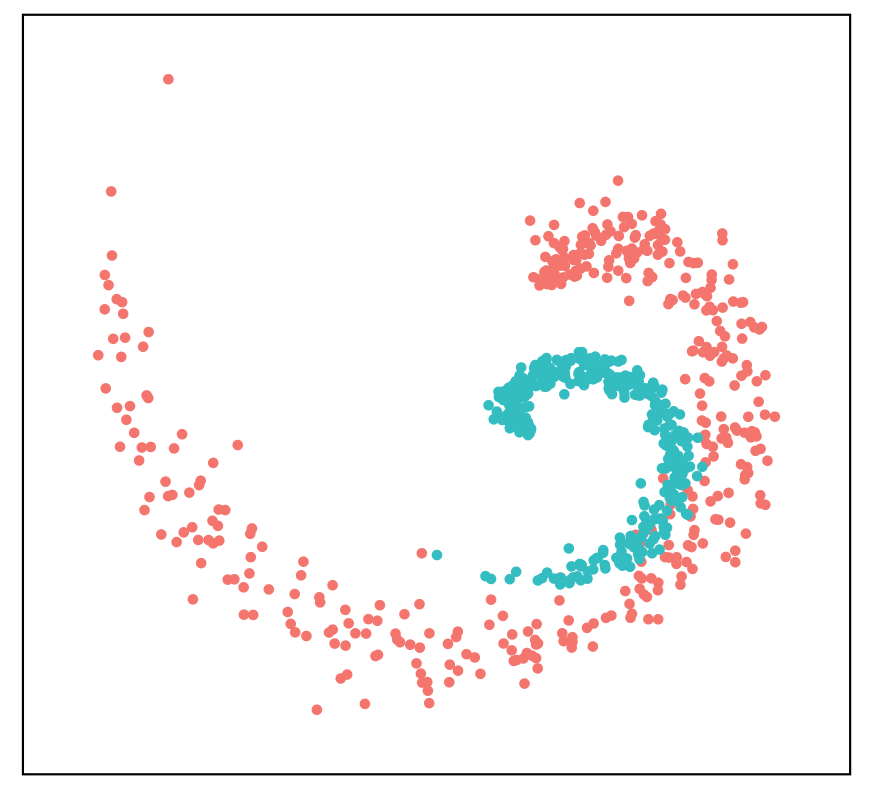
\includegraphics{figure/spiral_planar_data/data.png}}
      \tiny{\\ Credit : Ghatak, ch. 4}
      \caption{Simulated spiral planar data set with two classes.}
  \end{figure}
  \framebreak
  \begin{figure}
    \centering
      \scalebox{1}{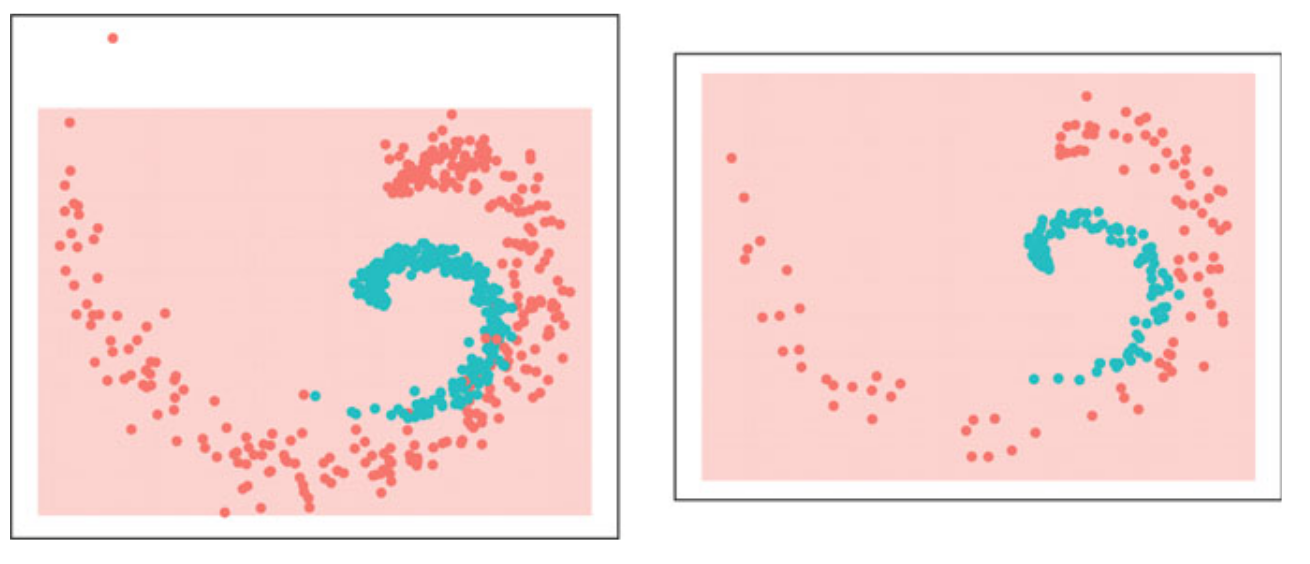
\includegraphics{figure/spiral_planar_data/zero.png}}
      \tiny{\\ Credit: Ghatak (2019), ch. 4}
      \caption{Decision boundary with zero initialization on the training data set (left) and the testing data set (right). The zero initialization does not break symmetry and the complexity of the network reduces to that of a single
neuron.}
  \end{figure}
    \framebreak
  \begin{figure}
    \centering
      \scalebox{1}{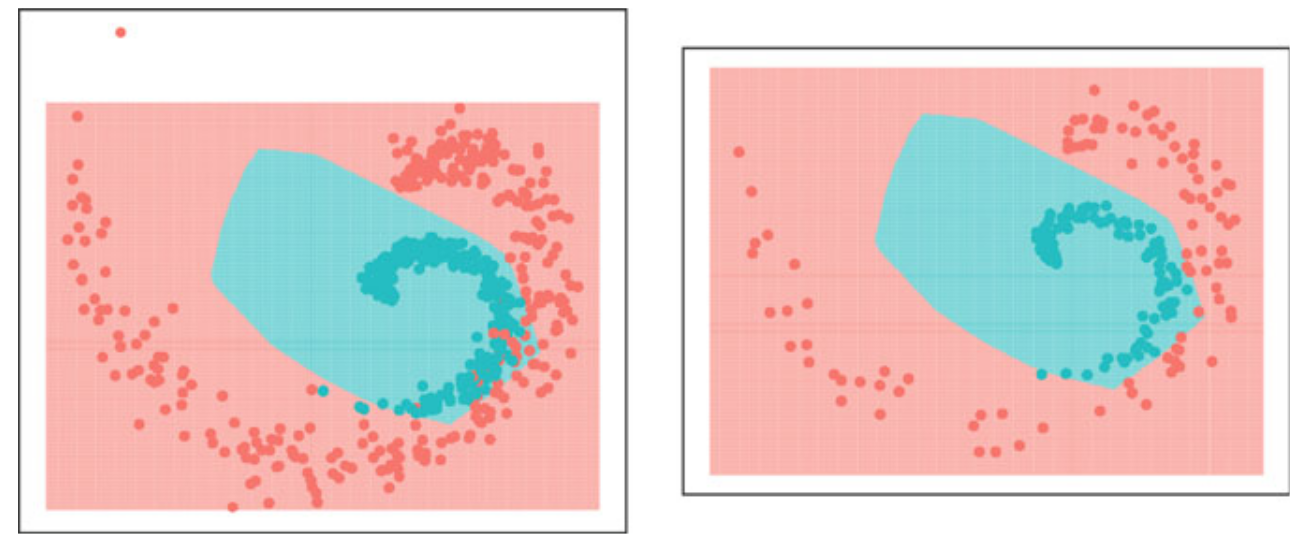
\includegraphics{figure/spiral_planar_data/random.png}}
      \tiny{\\ Credit: Ghatak (2019), ch. 4}
      \caption{Decision boundary with random initialization ($N\left(0, 1\cdot 10 ^{-4}\right)$) on the training data set (left) and the testing data set (right).}
  \end{figure}
      \framebreak
  \begin{figure}
    \centering
      \scalebox{1}{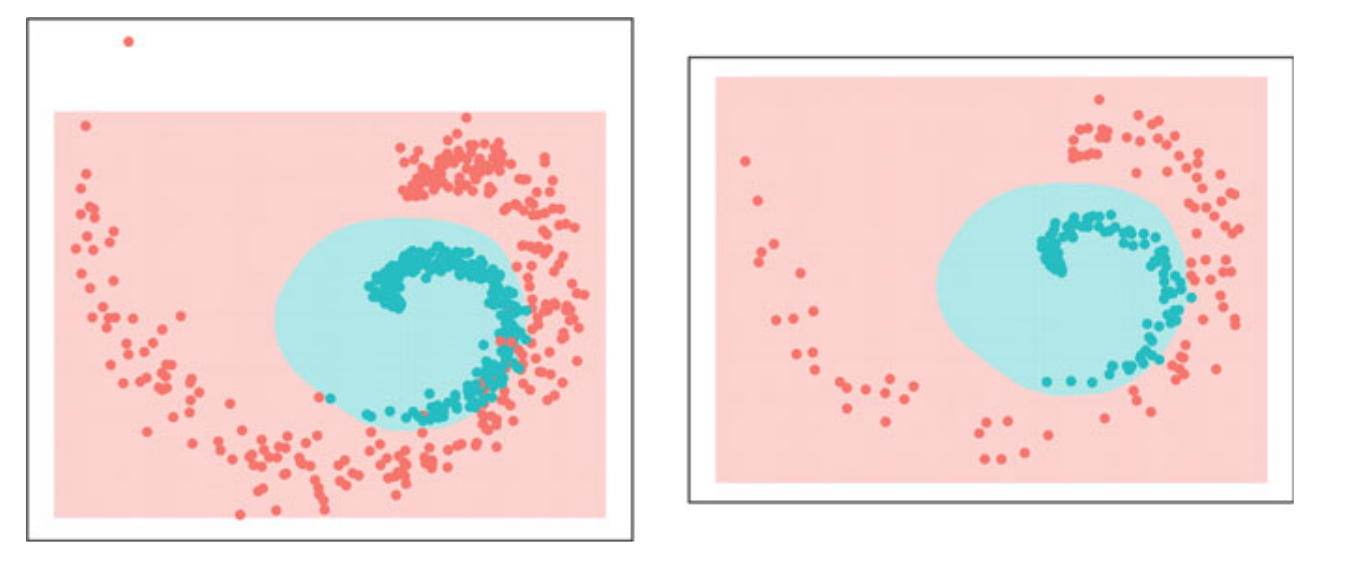
\includegraphics{figure/spiral_planar_data/he.png}}
      \tiny{\\ Credit: Ghatak (2019), ch. 4}
      \caption{Decision boundary with He initialization on the training data set (left) and the testing data set (right).}
  \end{figure}
\end{vbframe}

%%%%%%%%%%%%%%%%%%%%%%%%%%%%%%%%%%%%%%%%%%%%%%%%%%%%%%%%%%%%%%%%%%
\begin{vbframe}{Bias initialization}
  \begin{itemize}
    \item Typically, we set the biases for each unit to heuristically chosen constants. 
    \item Setting the biases to zero is compatible with most weight
initialization schemes as the schemes expect a small bias. 
    \item However, deviations from 0 can be made individually, for example, in order to obtain the right marginal statistics of the output unit or to avoid causing too much saturation at the initialization.
    \item For details see Goodfellow et. al (2016).
  \end{itemize}
\end{vbframe}



%%%%%%%%%%%%%%%%%%%%%%%%%%%%%%%%%%%%%%%%%%%%%%%%%%%%%%%%%%%%%%%%%%
%%%%%%%%%%%%%%%%%%          REFERENCES          %%%%%%%%%%%%%%%%%%
%%%%%%%%%%%%%%%%%%%%%%%%%%%%%%%%%%%%%%%%%%%%%%%%%%%%%%%%%%%%%%%%%%
\begin{vbframe}
\frametitle{References}
\footnotesize{
\begin{thebibliography}{99}
%%%%%%%%%%%%%%%%%%%%%%%%%%%%%%%%%%
\bibitem[Ian Goodfellow et al., 2016]{1} Ian Goodfellow, Yoshua Bengio and Aaron Courville (2016)
\newblock Deep Learning
\newblock \emph{\url{http://www.deeplearningbook.org/}}
%%%%%%%%%%%%%%%%%%%%%%%%%%%%%%%%%%
\bibitem[Kaiming He et. al., 2015]{1} Kaiming He, Xiangyu Zhang, Shaoqing Ren, and Jian Sun (2015)
\newblock Delving Deep into Rectifiers: Surpassing Human-Level Performance on ImageNet Classification. In Proceedings of the 2015 IEEE International Conference on Computer Vision (ICCV) (ICCV '15). IEEE Computer Society, Washington, DC, USA, 1026-1034. 
\newblock \emph{\url{https://arxiv.org/abs/1502.01852}}
%%%%%%%%%%%%%%%%%%%%%%%%%%%%%%%%%%
\bibitem[X. Glorot and Y. Bengio, 2010]{1} Xavier Glorot and Yoshua Bengio  (2010)
\newblock Understanding the difficulty of training deep feedforward neural networks AISTATS, Volume 9 von JMLR Proceedings, Seite 249-256. JMLR.org
\newblock \emph{\url{http://proceedings.mlr.press/v9/glorot10a/glorot10a.pdf?hc_location=ufi}}
%%%%%%%%%%%%%%%%%%%%%%%%%%%%%%%%%%%%
\bibitem[Abhijit Ghatak, 2019]{1} Abhijit Ghatak (2019)
\newblock Deep Learning with R. Springer.
%%%%%%%%%%%%%%%%%%%%%%%%%%%%%%%%%%
\end{thebibliography}
}
\end{vbframe}



%%%%%%%%%%%%%%%%%%%%%%%%%%%%%%%%%%%%%%%%%%%%%%%%%%%%%%%%%%%%%%%%%%
%%%%%%%%%%%%%%%%%%%%%%%%%%%%%%%%%%%%%%%%%%%%%%%%%%%%%%%%%%%%%%%%%%

\endlecture
\end{document}










